\documentclass[11pt]{article}

\usepackage[a4paper,margin=2.5cm]{geometry}
\usepackage{graphicx}
\usepackage{enumitem}
\usepackage{parskip}
\usepackage{xcolor}
\usepackage{titlesec}
\usepackage{hyperref}

\titleformat{\section}{\large\bfseries}{\thesection}{0.5em}{}
\titleformat{\subsection}{\normalsize\bfseries}{\thesubsection}{0.5em}{}

\title{\vspace{-1.5cm}\textbf{AW-01 User Manual}}
\author{}
\date{}

\begin{document}
\maketitle

\vspace{-1.5cm}

\textbf{AW-01} is an auto-wah plugin: a dynamic filter effect in which the center frequency of a filter is modulated by the amplitude envelope of the input signal. A louder input produces a different filter response than quieter input. The plugin's interface is organized into two main sections. The Envelope section controls how the input signal's envelope is detected and shaped (attack and decay times, and how strongly it drives the filter). The Filter section controls the characteristics of the filter itself (its cutoff/center frequency, resonance, and shape) that the envelope modulates. This document describes each parameter exposed by the plugin.

\begin{figure}[h!]
    \centering
    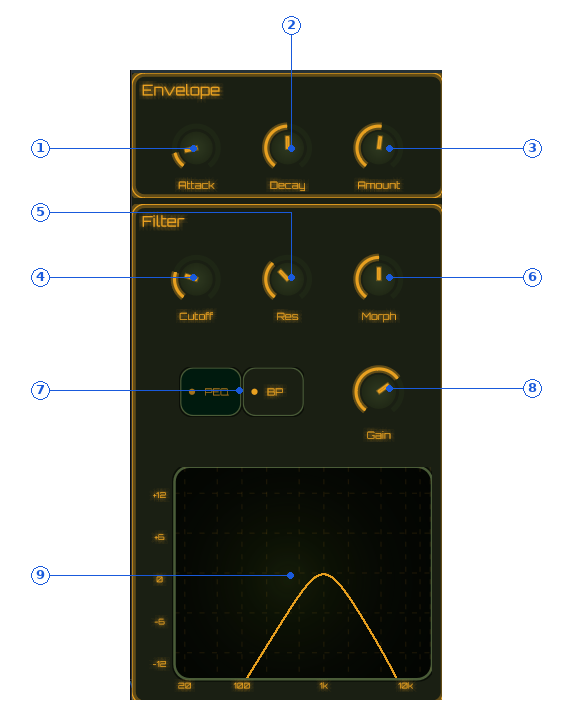
\includegraphics[width=0.9\textwidth]{annotated_v7.png}
    \caption{Plugin interface with numbered controls.}
    \label{fig:ui}
\end{figure}

\newpage

\begin{enumerate}[label=\textbf{\arabic*.}, leftmargin=2em]

\item \textbf{Attack} \\
Controls the time it takes for the envelope to rise from zero to its peak level after a note-on event. Higher values produce a slower onset. Lower values produce a sharp, percussive attack.

\item \textbf{Decay} \\
Controls the time it takes for the envelope to fall from its peak level down to the sustain level. Longer decay times produce a more gradual fade after the initial attack.


\item \textbf{Amount} \\
Sets the depth (modulation intensity) of the envelope's effect on the filter cutoff. At zero, the envelope has no audible effect; higher values increase the modulation depth.

\item \textbf{Cutoff} \\
Sets the corner (center) frequency of the filter. For the peaking EQ mode this is the frequency at which gain is applied; for the band-pass mode this is the center of the pass band.

\item \textbf{Res (Resonance)} \\
Controls the resonance (Q factor) of the filter around the cutoff frequency. Higher values narrow and emphasize the response around the cutoff, producing a more pronounced peak.

\item \textbf{Morph} \\
Morphs the filter's response between a low-pass or high-pass extreme and the mode set by the \textit{Filter Type} selector (item~7). Fully counterclockwise gives a low-pass response; fully clockwise gives a high-pass response; at center, the filter matches whichever mode (\textit{PEQ} or \textit{BP}) is currently selected. Intermediate knob positions blend continuously between the center mode and the nearest extreme.

\item \textbf{Filter Type (PEQ / BP selector)} \\
A single two-way selector that chooses the filter's operating mode: The two options are mutually exclusive, only one mode is active at a time.

\item \textbf{Gain} \\
Sets the amount of boost or cut applied by the filter when in \textit{PEQ} mode. Has no effect when the filter is in \textit{BP} mode.

\item \textbf{Frequency Response Display} \\
Graphical readout of the filter's current frequency response. The curve updates in real time as \textit{Cutoff}, \textit{Res}, \textit{Morph}, and \textit{Gain} are adjusted, providing visual feedback on the shape of the filter and its modulation.

\end{enumerate}

\section*{Code Signing Notice}

AW-01 is currently distributed \textbf{without code signing or notarization}. This is expected, and does not indicate a corrupted or malicious download.

\subsection*{Why isn't it signed?}

Code signing certificates (Apple Developer Program, Windows EV/OV certificates) require an ongoing paid subscription and, in Apple's case, notarization submission for every release. As an independently developed project, AW-01 does not currently carry these certificates. This does not affect the plugin's functionality, only the OS-level trust warnings shown on first launch.

\subsection*{macOS}

Since the installer and plugin binaries are not signed with an Apple Developer ID or notarized by Apple, macOS Gatekeeper will likely block the installer or plugin from opening on first launch, showing a warning
such as \textit{"AW-01 cannot be opened because the developer cannot be verified"} or \textit{"macOS cannot verify that this app is free from malware."}

To allow it to run, either:

\begin{enumerate}
    \item Right-click (or Control-click) the installer/plugin file, select \textbf{Open}, then confirm \textbf{Open} again in the dialog that appears; or

    \item Go to \textbf{System Settings} $\rightarrow$ \textbf{Privacy \& Security}, scroll to the Security section, and click \textbf{Open Anyway} next to the blocked item.
\end{enumerate}

This only needs to be done once per installed version.

\subsection*{Windows}

Similarly, since the installer is not signed with a Microsoft-trusted
code-signing certificate, Windows SmartScreen may display a
\textit{"Windows protected your PC"} warning when running the installer.

To proceed, click \textbf{More info}, then \textbf{Run anyway}.

\end{document}
